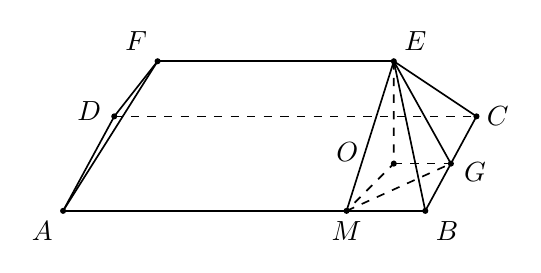
\begin{tikzpicture}[line width=0.6pt, font=\normalsize]
  \coordinate (A) at (0,0);
  \coordinate (B) at (4.6,0);
  \coordinate (M) at (3.6000000000,0.0000000000);
  \coordinate (D) at (0.6500000000,1.2000000000);
  \coordinate (C) at (5.2500000000,1.2000000000);
  \coordinate (F) at (1.2000000000,1.9000000000);
  \coordinate (E) at (4.2000000000,1.9000000000);
  \coordinate (O) at (4.2000000000,0.6000000000);
  \coordinate (G) at (4.9250000000,0.6000000000);
  % base and roof outlines
  \draw (A) -- (B);
  \draw (A) -- (D);
  \draw (A) -- (F);
  \draw (D)--(F);
  \draw (F) -- (E);
  \draw (E) -- (C);
  
  \draw (E) -- (B);
  \draw (E) -- (M);
  
  \draw (E) -- (G);
  
  \draw (B) -- (C);
  \draw[dashed] (D) -- (C);
  
  
  \draw[dashed] (O) -- (G);
  \draw[dashed] (M) -- (G);
  \foreach \p in {A,B,C,D,E,F,O,M,G} {\fill (\p) circle (1.1pt);}
  \node[below left=2pt, , inner sep=1.5pt] at (A) {$A$};
  \node[below right=2pt, , inner sep=1.5pt] at (B) {$B$};
  \node[right=2pt, , inner sep=1.5pt] at (C) {$C$};
  \node[left=3pt,yshift=2pt,inner sep=1.5pt] at (D) {$D$};
  \node[above right=2pt, , inner sep=1.5pt] at (E) {$E$};
  \node[above left=2pt, , inner sep=1.5pt] at (F) {$F$};
  \node[left=2pt, , inner sep=1.5pt,xshift=-9.034pt,yshift=4.015pt] at (O) {$O$};
  \node[below=2pt, , inner sep=1.5pt] at (M) {$M$};
  \node[right=2pt, , inner sep=1.5pt,xshift=1pt,yshift=-3pt] at (G) {$G$};
\draw[dashed] (E)--(O)--(M);
\end{tikzpicture}
